\newpage

\section{引言}

在本学期的物化实验课程中,我的主要收获总结如下:

\subsection{数据处理能力与报告撰写能力的提升}

在物化实验课程中,我通过处理实验数据和撰写实验报告,有效地提升了对Python的matplotlib, pandas, scipy, sympy, uncertainties等数据处理工具的熟练运用,同时也掌握了利用Origin进行辅助作图和使用LaTeX编写实验报告的技能。这些重要的软件和工具的使用已经变得我非常熟悉。通过每周一次的实验报告写作练习,我的报告撰写技巧得到了显著提高,不仅在规范性上有所加强,而且在撰写速度上也有了明显的提升。这些在物化实验课程中积累的经验将对我未来的科研工作带来积极的助益。

\subsection{实验操作与实验设计能力的进步}

在物化实验课程中,我得以将物理化学理论课程中学习的知识应用到实际实验中,进而深化了我对物化理论的理解。这一过程完美展现了化学作为一门实验科学的本质,即理论和实验相互补充、相辅相成的特性。

课程中的许多经典实验,如燃烧热和溶解热实验,都展现了精妙的实验设计思路。这些实验通常使用简单的装置,结合恰当的数据处理方法,便能获得相当精确的结果。通过学习这些实验设计,我获得了丰富的知识和经验,对我的学术发展大有裨益。


\section{物化实验课程的意见和建议}

尽管撰写物化实验报告对于提升学生的能力具有显著效果,但每周需提交一篇实验报告的要求在很多情况下给学生每周的学习时间安排带来了相当大的压力。这导致了选修此课程的学生不得不投入大量时间于实验报告的编写,从而在很大程度上减少了他们用于学习其他课程的可用时间。本学期虽然开始尝试将实验报告分为简写版与详写版,但根据我个人的经验而言,这几乎没有改变我的报告撰写时间,主要时间仍然消耗在数据处理之上,而非结果讨论。

希望物理化学实验的老师,要搞清楚物理化学实验的定位只是一个3学分的化学学院专业课,一周理应消耗在其上的时间小于6小时,也就是说报告撰写的期望时间是2-4小时才合适,而根据我的观察与统计,单单完成一份报告撰写至少需要7小时以上,这对课程定位而言无疑是极其不合理的。这样过度集中于报告撰写的课程对学生而言更多是一种重复性的过度训练,而其边际效益早已随着过度重复的报告撰写递减至一个相当低的程度。

如果北大化院就是想要开设一门锻炼同学们学术报告撰写和科学数据处理的课程,不如将《物化实验》改成《物化实验报告撰写》,取消所有实验室的环节,仅保留报告撰写部分;如果化院还想训练同学们的实验能力,请优化实验-报告时间和评分的安排,而不是从两方面都给予学生压力,这无疑会造成学生们的身心伤害:据我的经历和实验授课老师的反映,有相当多的同学需要熬一个或半个通宵来完成实验报告的撰写。这也从一份关于化学院同学的睡眠质量调查得以侧面印证,如图 \ref{fig:1}。

\begin{figure}[htbp]
    \centering
    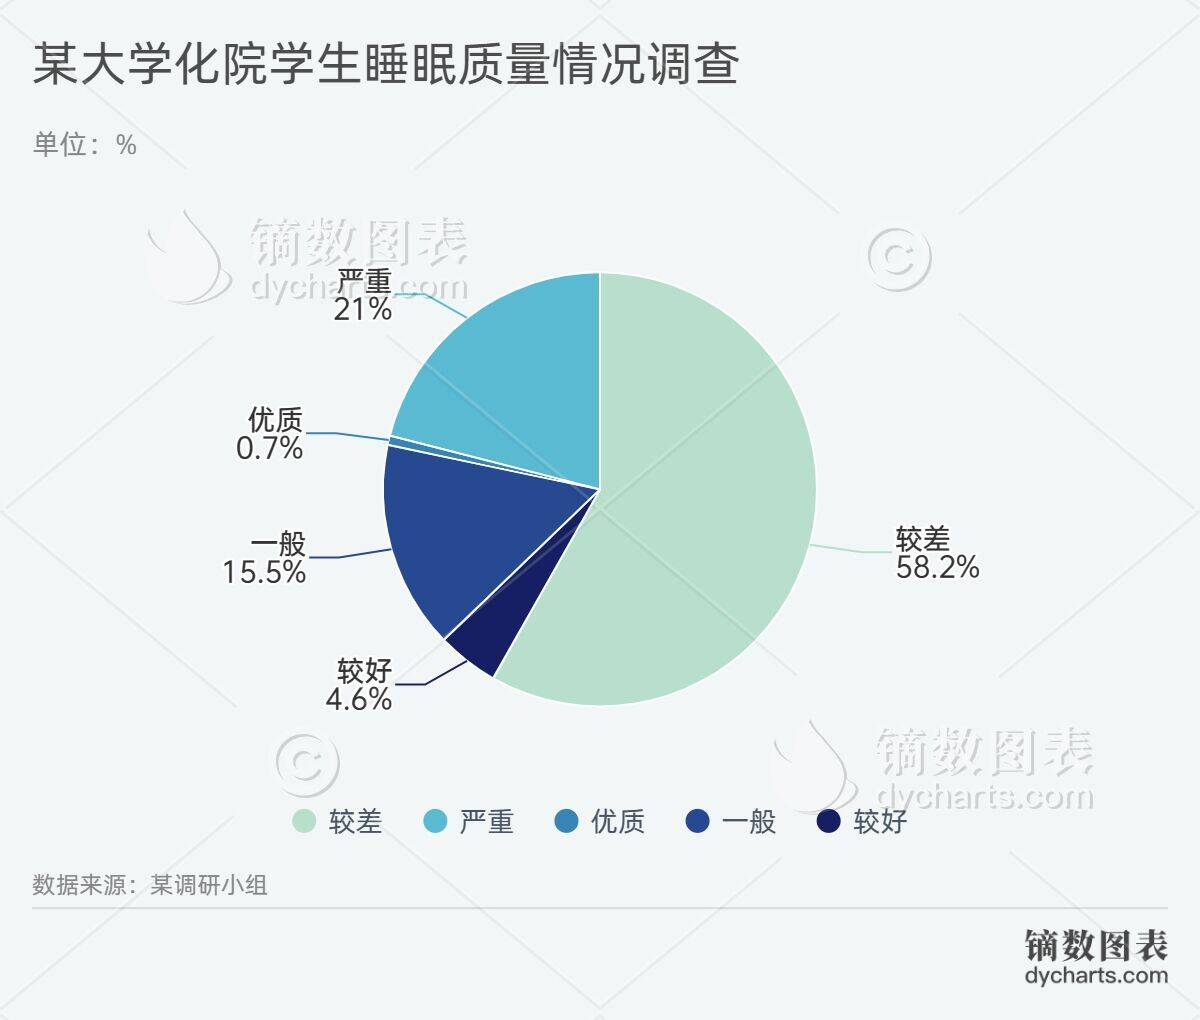
\includegraphics[width=.7\textwidth]{figures/1.jpg}
    \caption{某小组进行的北大各个学院睡眠质量调查统计}
    \label{fig:1}
\end{figure}

我们同学也是人,也希望在北京大学化学院得到和人一样的待遇与尊重,从这里我们希望收货知识,而不是一幅残破的身躯与失业的境遇。我奉劝各位老师:\textbf{如果你们真的希望化院好的话,那就请善待自己的学生,多一点包容,少一点苛求}。

现在中国青年失业率高企(官方截止去年8月为22\%,之后便停止公布该数据,而北京大学张丹丹副教授估计去年3月份失业率已达46.5\%),在这种形势下,对于所谓“天坑专业”的化学专业的就业情况更不乐观。在这种压力下,希望老师们能够多给同学们一点时间培养一些对自己有用的技能,而不是把同学们的时间都耗在意义甚微的重复劳动上。

我们同学们也会像化院爱我们一样,热爱着化院!

\section{其他同学的评价}

借这个为数不多的机会,我想向老师展示以为前化院同学的评价。

“有感而发,谈谈我对化院的看法。

“首先,化院的目的决定了它不是一个学习知识的地方,而是一个教化场所,承担着再社会化的职能,将学科范式(而不是知识)灌输给学生,以期达到它的根本目的:培养本行业需要的人才(以及给化院众多在编人员吃饭)。

“大部分高中的目的是高考(此目的根据学生家庭情况有强弱之分),故其训练皆针对高考模式,从上课的讲义,到课本习题,到模拟押题卷,本质上是范式的训练。从小学到高中的范式转移也并非革命性的变化,小升初,中考,高考具有一定的相似性,这种不变性构成了义务教育阶段我们对“学习”的概念,故小升初,初升高鲜少有结构性矛盾导致无法适应的出现(国际学校,贵族学校等除外),而多见暂时的适应困难。

“而及至大学(具体来说,化院),惯性被打破,学术科研的新范式骤然降临,带来无法解决的结构性矛盾:科学已然不是堂吉诃德侠义骑士的黄金时代,单枪匹马的传奇只能折戟沉沙,我们必须可悲地承认,化学的研究范式需要大量线列步兵填补战线。而线列步兵是不应该花天酒地的,战斗不息,他只能一刻不停。

“是故,在化院课堂传授知识的表象下,隐藏着框定生活模式的职能。

“许多同学曾抱怨,自己作为竞赛生/有竞赛基础的学生,其实并不能在课堂上学到什么新知识,却不得不写着大量作业,准备各式各样的论文。其实这并不意外,化院的目的是框定生活模式,换句话说是训练,而没有比齐步走更有效的训练了,难道你还指望在齐步走中学习什么先进的军事理论吗?训练总是机械的,无意义的重复。在此意义上,化院的课程设置不可谓不成功。
而实验课,更是这种教化思想指导下的登峰造极之作。经过半天的实验课,你还想着阅读,批判,分析,思辨么?不如倒头就睡,明天醒来又是一个崭新的化院人。

“这种半强制性体制的最大危机不是合法性(合法性由权威与传统共同授予),而是稳定性,经过小范围调查,保守估计本届化院想润者十有五六,这种潜在的危机需要制度性保障与非制度性因素共同作用来避免。很显然,前者大名“强基计划”,而后者,请看化院均绩在全校的排名(笑)

“写到此,我不由得振臂高呼!“不要问化院能为你做什么,而去问你能为花园做什么”,在一门门乏味的课程中,化院的利维坦正伸出触手。在每个不眠的奋斗之夜,在每瓶酚酞变红之时,在每锅反应终始之刻,你都在与不可名状的集体意志做着危险的互动,他将会逐滴剥夺你的人性,就像滴定剂消逝于漩涡中,打工仔异化于富士康的集体宿舍,本科生迷茫于蚊虫纷扰的三十六号楼。这个过程缓慢而无法察觉,绝望却无可逆转。不要问及重复劳动的意义,不要问及给分的随机性,不要问及连珠般的考试,神现在告诉你:“耶稣,祂为你而来,祂为我们而来!” ”

\section{解决实验压力:数据开源计划}

当前互联网时代下,开源无疑是一股强劲的潮流,将资源开源化已成为诸多科研项目的共识,例如目前诸多出版商都在推出Open-Access期刊,以促进科学对普通人的普及与科研的交流。

我认为如果老师们不想减少物理化学实验的任务量,实行数据开源计划是一种非常科学的方案,据我的观察,同学们每人都有至少一份学长的报告,这对我们的实验报告撰写给予了巨大的便利。因此,我计划从我做起,将实验报告完全开源,包括数据处理过程的代码与实验报告的Latex源文件。我将会将项目经过简单的处理,陆续上传至Github,也欢迎老师同学们的访问与监督。
